% Options for packages loaded elsewhere
\PassOptionsToPackage{unicode}{hyperref}
\PassOptionsToPackage{hyphens}{url}
%
\documentclass[
  letterpaper,
  ignorenonframetext,
  aspectratio=43,
  handout,
  12pt]{beamer}
\usepackage{pgfpages}
\setbeamertemplate{caption}[numbered]
\setbeamertemplate{caption label separator}{: }
\setbeamercolor{caption name}{fg=normal text.fg}
\beamertemplatenavigationsymbolsempty
% Prevent slide breaks in the middle of a paragraph
\widowpenalties 1 10000
\raggedbottom
\setbeamertemplate{part page}{
  \centering
  \begin{beamercolorbox}[sep=16pt,center]{part title}
    \usebeamerfont{part title}\insertpart\par
  \end{beamercolorbox}
}
\setbeamertemplate{section page}{
  \centering
  \begin{beamercolorbox}[sep=12pt,center]{part title}
    \usebeamerfont{section title}\insertsection\par
  \end{beamercolorbox}
}
\setbeamertemplate{subsection page}{
  \centering
  \begin{beamercolorbox}[sep=8pt,center]{part title}
    \usebeamerfont{subsection title}\insertsubsection\par
  \end{beamercolorbox}
}
\AtBeginPart{
  \frame{\partpage}
}
\AtBeginSection{
  \ifbibliography
  \else
    \frame{\sectionpage}
  \fi
}
\AtBeginSubsection{
  \frame{\subsectionpage}
}
\usepackage{amsmath,amssymb}
\usepackage{lmodern}
\usepackage{iftex}
\ifPDFTeX
  \usepackage[T1]{fontenc}
  \usepackage[utf8]{inputenc}
  \usepackage{textcomp} % provide euro and other symbols
\else % if luatex or xetex
  \usepackage{unicode-math}
  \defaultfontfeatures{Scale=MatchLowercase}
  \defaultfontfeatures[\rmfamily]{Ligatures=TeX,Scale=1}
\fi
\usetheme[]{metropolis}
% Use upquote if available, for straight quotes in verbatim environments
\IfFileExists{upquote.sty}{\usepackage{upquote}}{}
\IfFileExists{microtype.sty}{% use microtype if available
  \usepackage[]{microtype}
  \UseMicrotypeSet[protrusion]{basicmath} % disable protrusion for tt fonts
}{}
\makeatletter
\@ifundefined{KOMAClassName}{% if non-KOMA class
  \IfFileExists{parskip.sty}{%
    \usepackage{parskip}
  }{% else
    \setlength{\parindent}{0pt}
    \setlength{\parskip}{6pt plus 2pt minus 1pt}}
}{% if KOMA class
  \KOMAoptions{parskip=half}}
\makeatother
\usepackage{xcolor}
\IfFileExists{xurl.sty}{\usepackage{xurl}}{} % add URL line breaks if available
\IfFileExists{bookmark.sty}{\usepackage{bookmark}}{\usepackage{hyperref}}
\hypersetup{
  hidelinks,
  pdfcreator={LaTeX via pandoc}}
\urlstyle{same} % disable monospaced font for URLs
\newif\ifbibliography
\usepackage{graphicx}
\makeatletter
\def\maxwidth{\ifdim\Gin@nat@width>\linewidth\linewidth\else\Gin@nat@width\fi}
\def\maxheight{\ifdim\Gin@nat@height>\textheight\textheight\else\Gin@nat@height\fi}
\makeatother
% Scale images if necessary, so that they will not overflow the page
% margins by default, and it is still possible to overwrite the defaults
% using explicit options in \includegraphics[width, height, ...]{}
\setkeys{Gin}{width=\maxwidth,height=\maxheight,keepaspectratio}
% Set default figure placement to htbp
\makeatletter
\def\fps@figure{htbp}
\makeatother
% Make links footnotes instead of hotlinks:
\DeclareRobustCommand{\href}[2]{#2\footnote{\url{#1}}}
\setlength{\emergencystretch}{3em} % prevent overfull lines
\providecommand{\tightlist}{%
  \setlength{\itemsep}{0pt}\setlength{\parskip}{0pt}}
\setcounter{secnumdepth}{-\maxdimen} % remove section numbering
\usepackage{pgfpages}
\pgfpagesuselayout{2 on 1}
\providecommand{\tightlist}{%
\setlength{\itemsep}{0pt}\setlength{\parskip}{0pt}}
\makeatletter
\makeatother
\let\Oldincludegraphics\includegraphics
\renewcommand{\includegraphics}[2][]{\Oldincludegraphics[width=\textwidth,height=0.7\textheight,keepaspectratio]{#2}}
\ifLuaTeX
  \usepackage{selnolig}  % disable illegal ligatures
\fi

\author{}
\date{}

\begin{document}

\begin{frame}
Lecture 16 - Damage Theory

Dr.~Nicholas Smith

Wichita State University, Department of Aerospace Engineering

April 1, 2021
\end{frame}

\begin{frame}{schedule}
\protect\hypertarget{schedule}{}
\begin{itemize}
\tightlist
\item
  Apr 1 - Damage Theory
\item
  Apr 6 - Damage Theory
\item
  Apr 8 - Dislocation Theory
\item
  Project Work Days
\end{itemize}
\end{frame}

\begin{frame}{outline}
\protect\hypertarget{outline}{}
\begin{itemize}
\tightlist
\item
  failure
\item
  spherical void growth
\item
  cylindrical void growth
\item
  micro cracks
\end{itemize}
\end{frame}

\hypertarget{failure}{%
\section{failure}\label{failure}}

\begin{frame}{failure}
\protect\hypertarget{failure-1}{}
\begin{itemize}
\tightlist
\item
  Ductile fracture

  \begin{itemize}
  \tightlist
  \item
    plastic deformation prior to failure
  \item
    dimpled, cup and cone fracture surface
  \end{itemize}
\item
  Brittle fracture

  \begin{itemize}
  \tightlist
  \item
    rapid crack propagation
  \item
    generally flat fracture surface
  \item
    common in glasses, thermoset polymers, brittle metals (BCC and HCP
    crystals)
  \end{itemize}
\end{itemize}
\end{frame}

\begin{frame}{fracture surface}
\protect\hypertarget{fracture-surface}{}
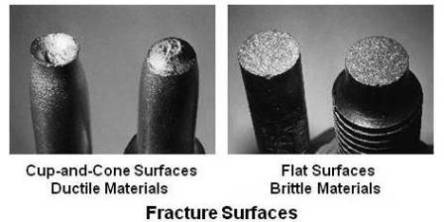
\includegraphics{../images/Fracture-Surfaces-.jpg}
\end{frame}

\begin{frame}{ductile fracture surface}
\protect\hypertarget{ductile-fracture-surface}{}
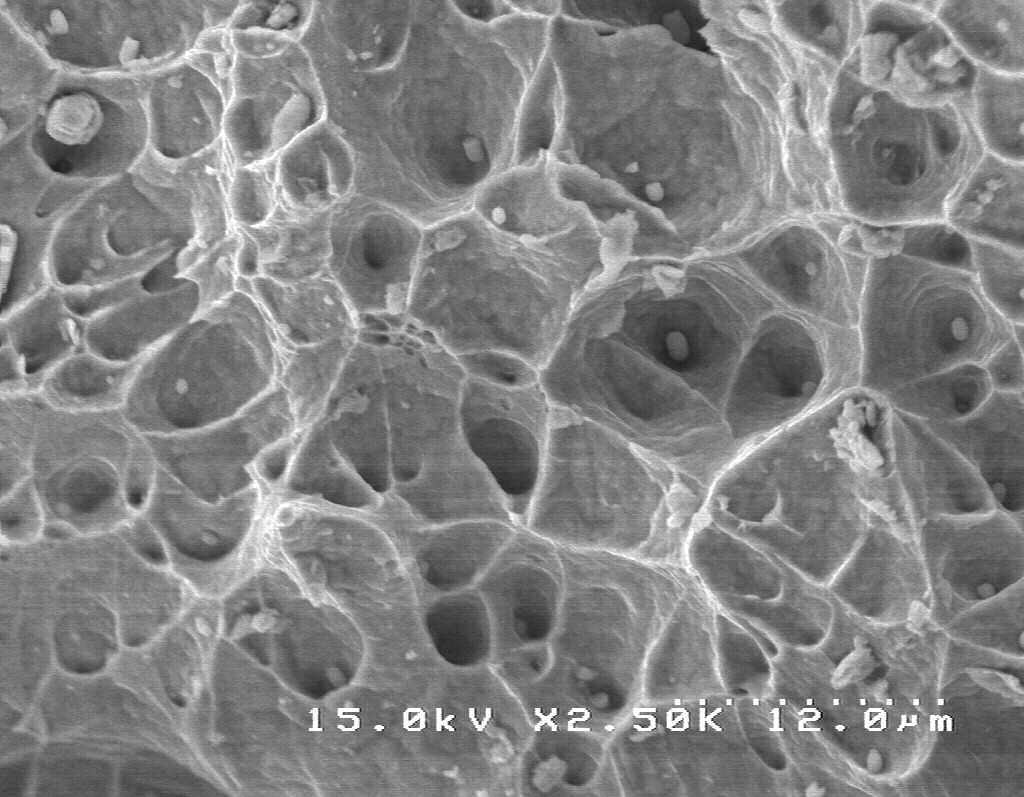
\includegraphics{../images/ductile1.jpg}
\end{frame}

\begin{frame}{ductile fracture surface}
\protect\hypertarget{ductile-fracture-surface-1}{}
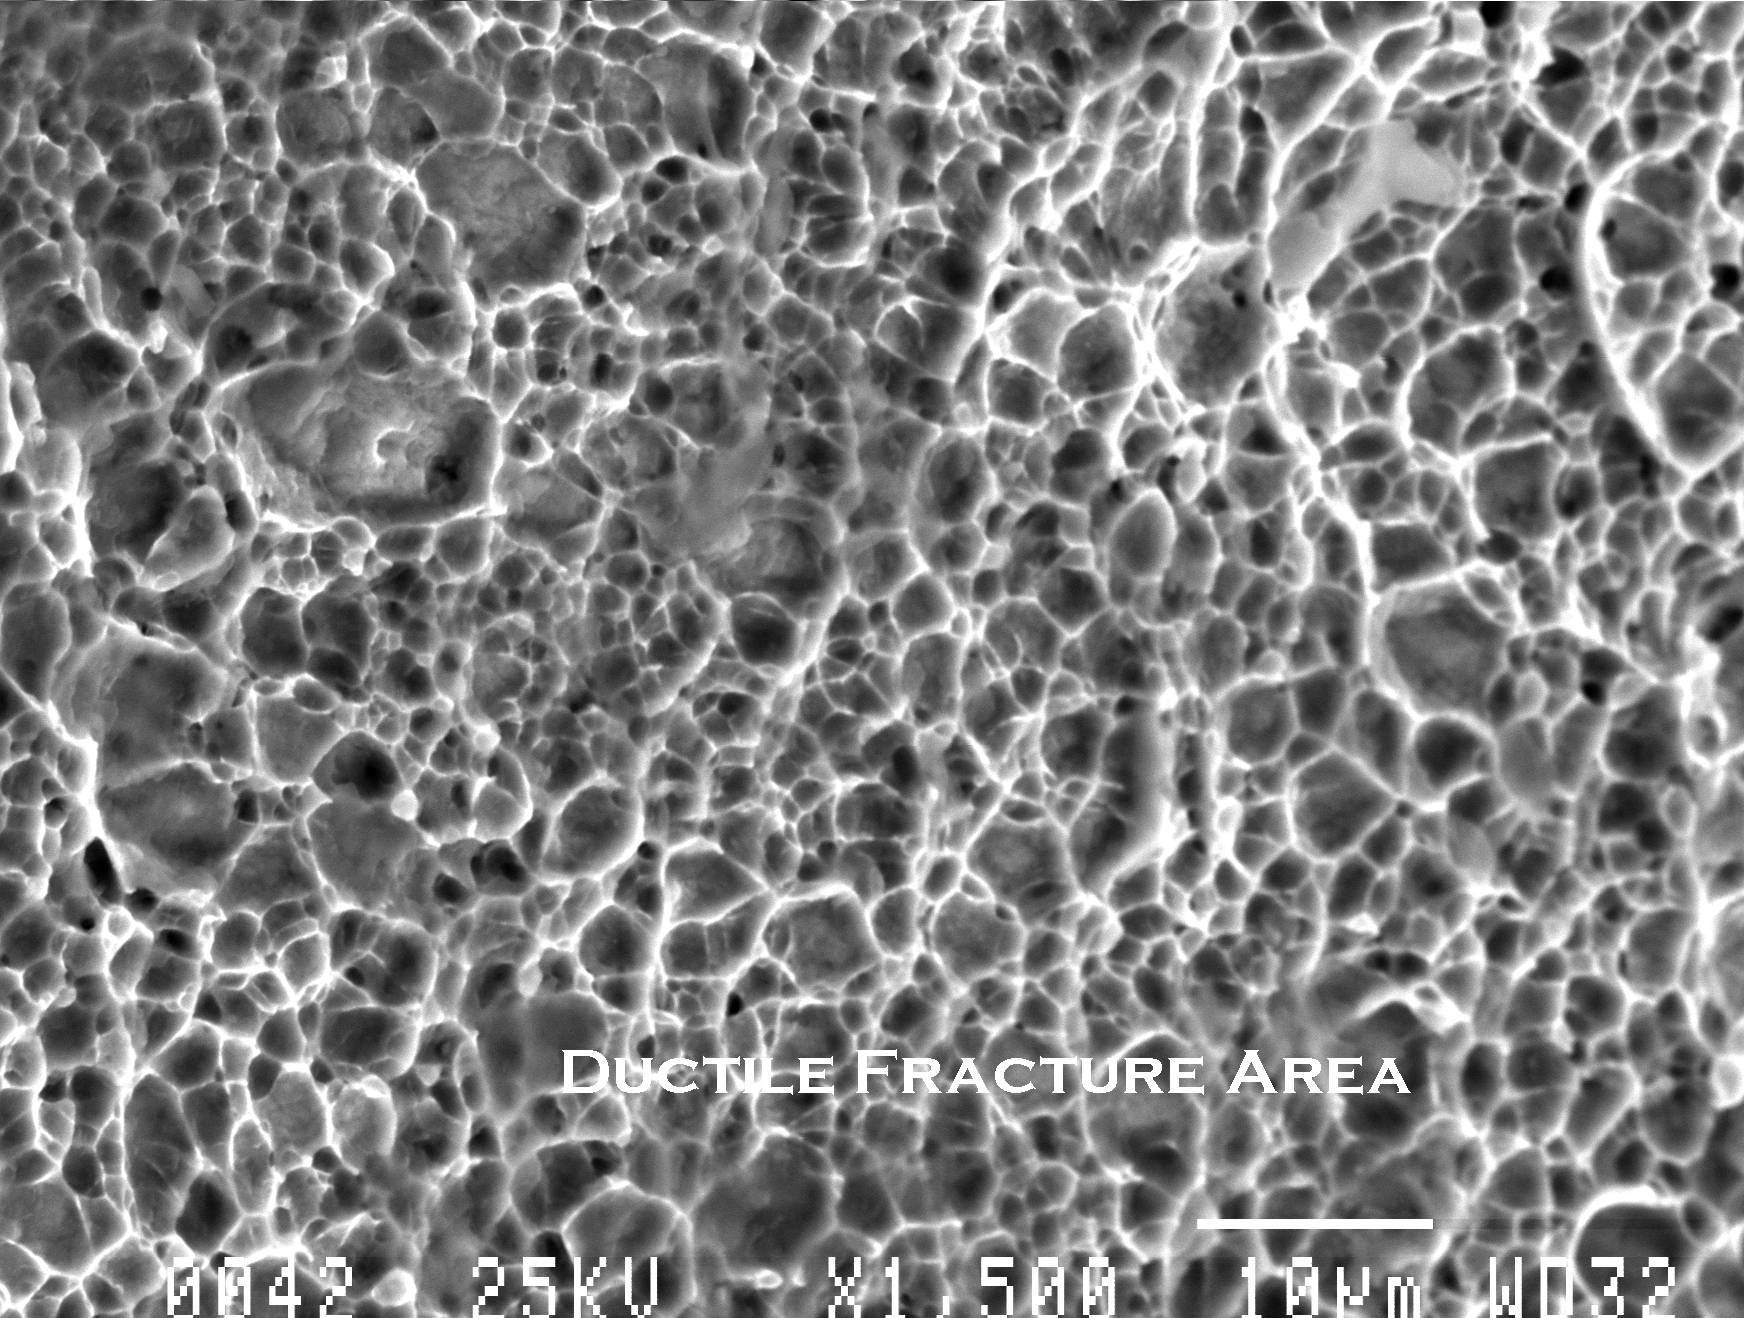
\includegraphics{../images/ductile2.jpg}
\end{frame}

\begin{frame}{brittle fracture surface}
\protect\hypertarget{brittle-fracture-surface}{}
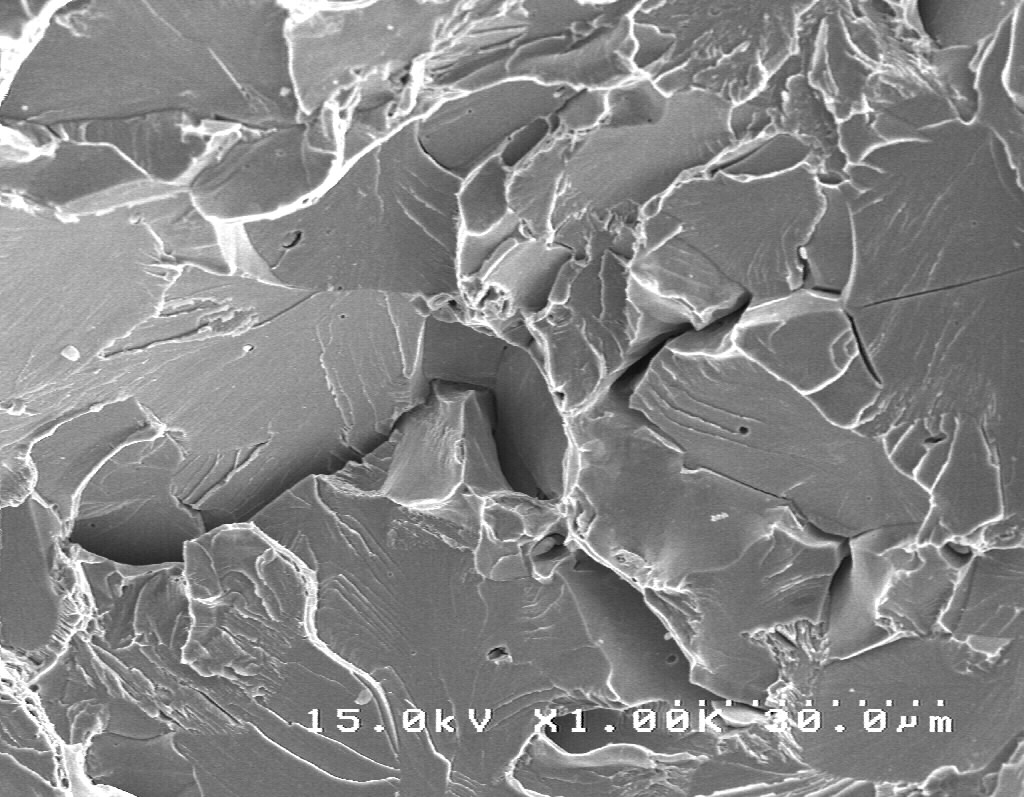
\includegraphics{../images/brittle1.jpg}
\end{frame}

\begin{frame}{brittle fracture surface}
\protect\hypertarget{brittle-fracture-surface-1}{}
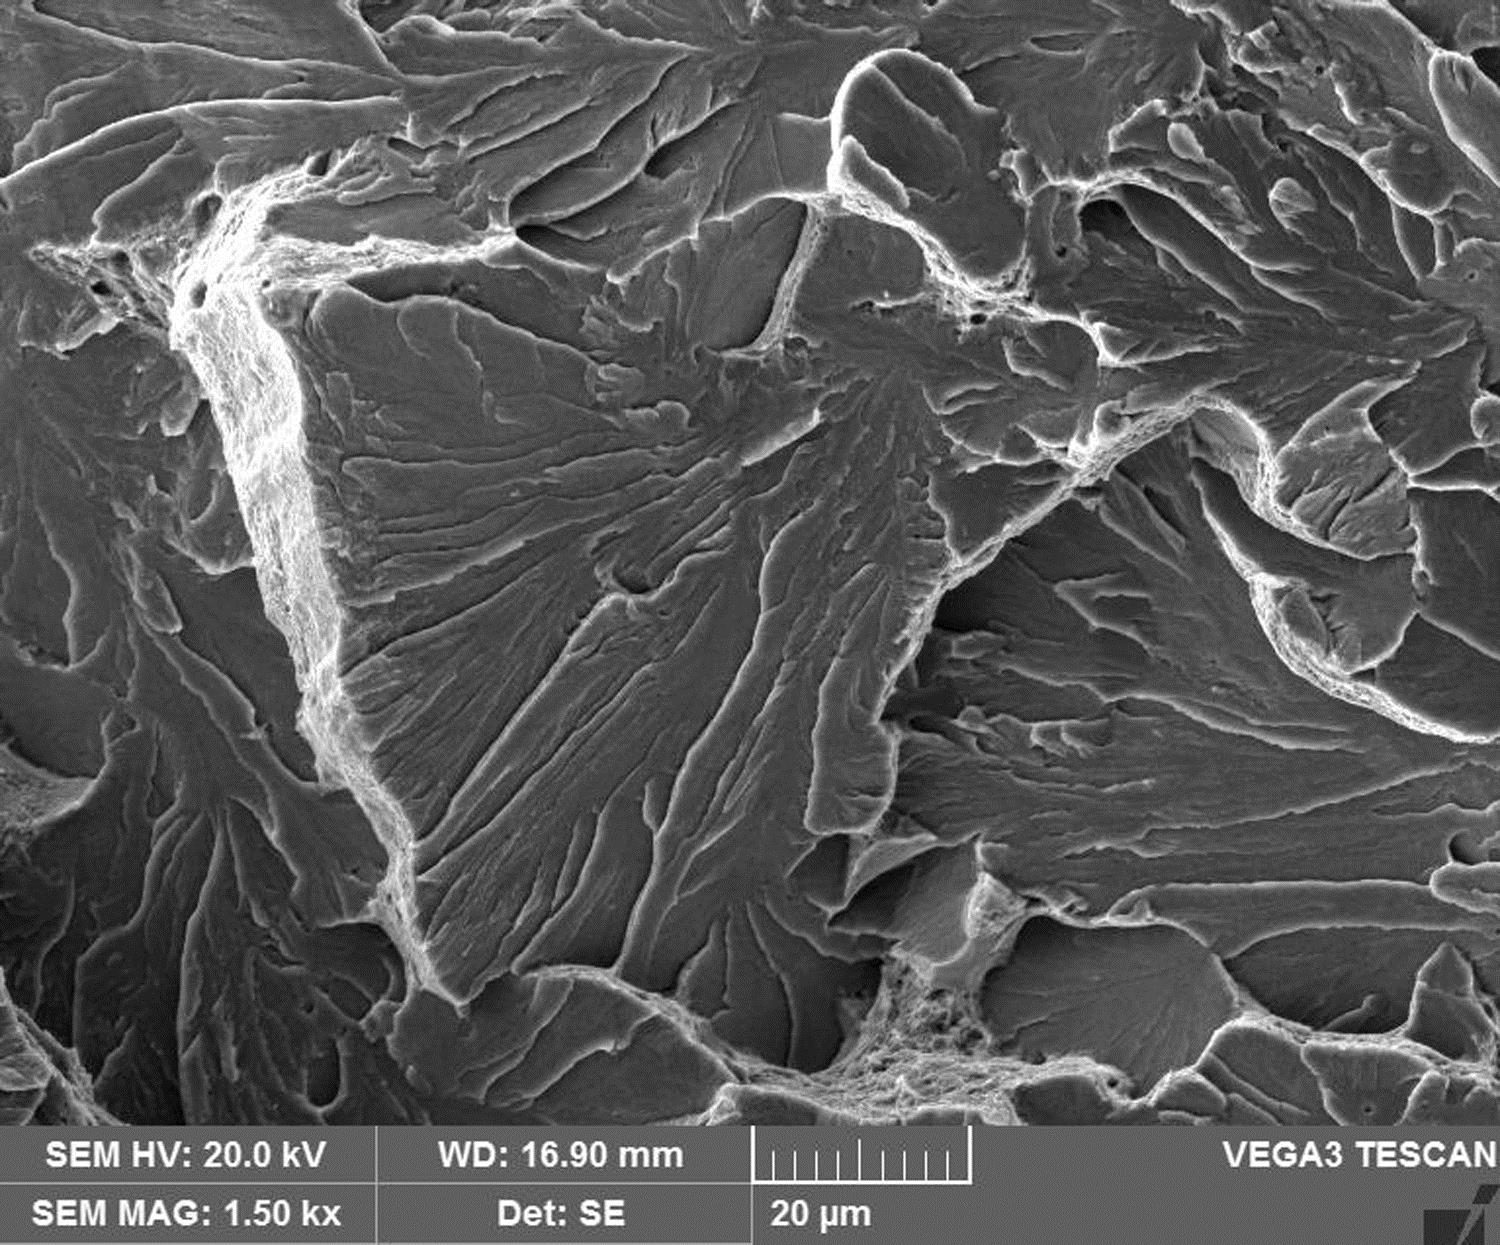
\includegraphics{../images/brittle2.jpg}
\end{frame}

\begin{frame}{transition}
\protect\hypertarget{transition}{}
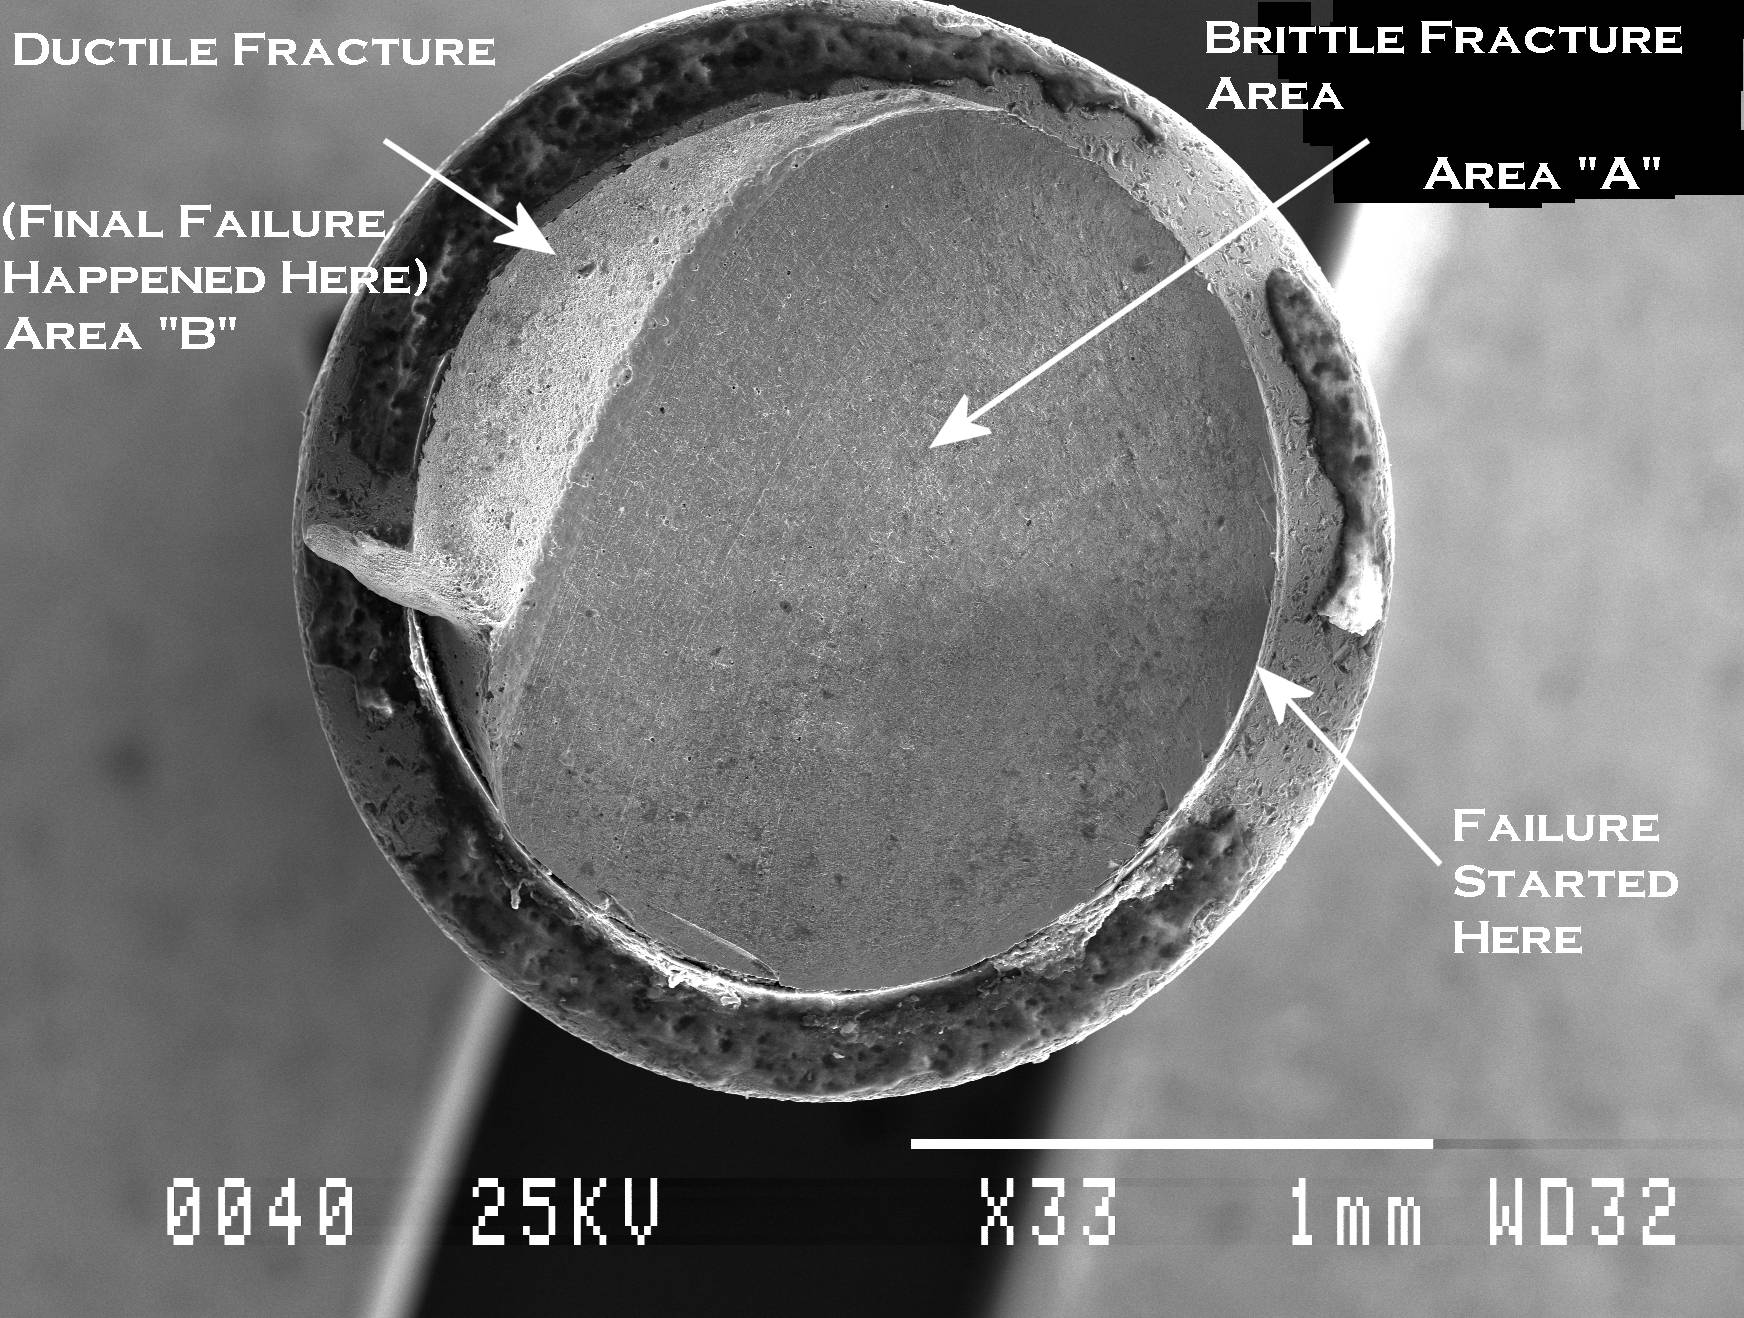
\includegraphics{../images/transition.jpg}
\end{frame}

\begin{frame}{what affects failure method}
\protect\hypertarget{what-affects-failure-method}{}
\begin{itemize}
\tightlist
\item
  While some materials are generally ductile or brittle, there are
  factors that can cause brittle failure in a ductile material
\item
  Strain rate (materials are often more brittle at high strain rates)
\item
  Temperature also affects ductility of many materials
\end{itemize}
\end{frame}

\begin{frame}{temperature effects}
\protect\hypertarget{temperature-effects}{}
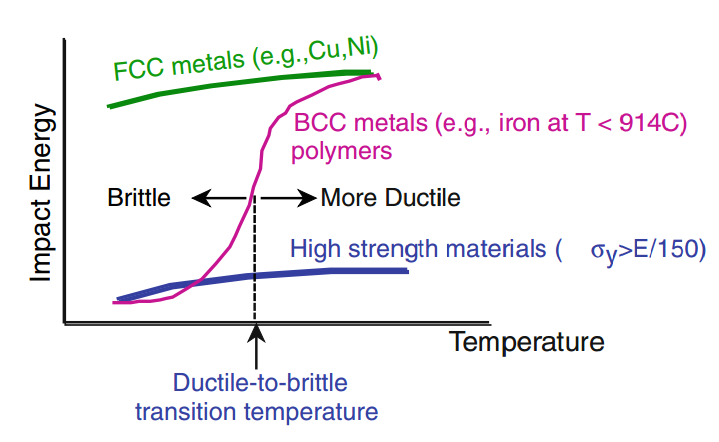
\includegraphics{../images/temperature.PNG}
\end{frame}

\hypertarget{spherical-void-growth}{%
\section{spherical void growth}\label{spherical-void-growth}}

\begin{frame}{void growth}
\protect\hypertarget{void-growth}{}
\begin{itemize}
\tightlist
\item
  From what we have observed on fracture surfaces, it appears that
  ductile materials fail due to void growth
\item
  Some of the earliest and simplest micromechanical damage models are
  for spherical void growth
\item
  Spherical voids are typical of uniaxial tension
\end{itemize}
\end{frame}

\begin{frame}{spherical voids in viscous materials}
\protect\hypertarget{spherical-voids-in-viscous-materials}{}
\begin{itemize}
\tightlist
\item
  If we consider a spherical void in a linear, viscous RVE under some
  uniform remote stress, \(\sigma^\infty\) the constitutive behavior is
\end{itemize}

\[\sigma_{ij} = L_{ijkl}\dot{\epsilon}_{kl}\]

\begin{itemize}
\tightlist
\item
  \emph{L} is analogous to the stiffness tensor, but relates stress to
  strain-rate
\item
  For an isotropic material, we can define \emph{L} in terms of \(\eta\)
  and \(\nu\) to give the familiar relationshiop
\end{itemize}

\[\sigma_{ij} = 2\eta \left(\dot{\epsilon}_{ij}+\frac{\nu}{1-2\nu} \dot{\epsilon}_{kk}\delta_{ij}\right)\]
\end{frame}

\begin{frame}{spherical voids in viscous materials}
\protect\hypertarget{spherical-voids-in-viscous-materials-1}{}
\begin{itemize}
\tightlist
\item
  Eshelby's model holds true for a viscous material as well as a solid,
  so we can find the stress inside the void as
\end{itemize}

\[\sigma_{ij} = L_{ijkl}\left(\dot{\epsilon}_{kl}^\infty + \dot{\epsilon}_{kl}^d - \dot{\epsilon}_{kl}^*\right)\]

\begin{itemize}
\tightlist
\item
  But we know that there is no stress inside the void, thus we can say
\end{itemize}

\[\dot{\epsilon}_{kl}^\infty + \dot{\epsilon}_{kl}^d - \dot{\epsilon}_{kl}^* = 0\]

\begin{itemize}
\tightlist
\item
  Where, in this case, \(\dot{\epsilon}_{kl}^*\) is the strain-rate of
  the void
\end{itemize}
\end{frame}

\begin{frame}{spherical voids in viscous materials}
\protect\hypertarget{spherical-voids-in-viscous-materials-2}{}
\begin{itemize}
\tightlist
\item
  pp.~266-267 in the text show the details for calculating the Eshelby
  tensor with a spherical void
\item
  However, when a non-uniform load is applied (uni-axial or biaxial
  tension) the void will no longer be spherical
\item
  Also, there are not many solids that can be adequately described with
  a linearly viscous constitutive law
\end{itemize}
\end{frame}

\hypertarget{cylindrical-void-growth}{%
\section{cylindrical void growth}\label{cylindrical-void-growth}}

\begin{frame}{mcclintock solution}
\protect\hypertarget{mcclintock-solution}{}
\begin{itemize}
\tightlist
\item
  McClintock developed the first widely-accepted void growth model
\item
  He assumed a cylindrical void shape (for tension along the cylinder
  axis)
\item
  He assumed the material surrounding the void was incompressible,
  rigid-plastic
\item
  In spite of the simplifications made, this model has served as a
  benchmark for many homogeneous schemes.
\end{itemize}
\end{frame}

\begin{frame}{mcclintock solution}
\protect\hypertarget{mcclintock-solution-1}{}
\begin{itemize}
\tightlist
\item
  To date, the mcClintock solution is the only exact analytic solution
  for void growth in non-linear solids
\item
  A full derivation, for some assumptions in yield criterion and plastic
  flow rule is in text pp.~268-271
\end{itemize}
\end{frame}

\begin{frame}{mcclintock solution}
\protect\hypertarget{mcclintock-solution-2}{}
\begin{itemize}
\tightlist
\item
  For the Von Mises (J2) yield criterion and the flow rule defined on
  p.~268, we find
\end{itemize}

\[\frac{\dot{a}}{a} = \frac{\sqrt{3}}{2}|\dot{\epsilon}_z| \sinh \left(\frac{\sqrt{3}\sigma^\infty}{\sigma_{YS}}\right) - \frac{1}{2} \dot{\epsilon}_z\]

\begin{itemize}
\tightlist
\item
  McClintock predicts that void growth increases exponentially with
  applied stress, while the linear viscous solution predicts a linear
  relationship between void growth and stress
\end{itemize}
\end{frame}

\begin{frame}{mcclintock solution}
\protect\hypertarget{mcclintock-solution-3}{}
\begin{itemize}
\tightlist
\item
  Many damage models use the volume fraction of voids
\item
  In the McClintock solution, the matrix is considered incompressible
\item
  This means we can write the rate of change of volume fraction as
\end{itemize}

\[\dot{f} = \sqrt{3} f (1-f) |\dot{\epsilon}_z|\sinh\left(\frac{\sqrt{3}\sigma_{11}}{|\sigma_{33}-\sigma_{11}|}\right)\]
\end{frame}

\begin{frame}{gurson model}
\protect\hypertarget{gurson-model}{}
\begin{itemize}
\tightlist
\item
  Gurson's model builds on McClintock's solution
\item
  He homegenizes the micro-stress to define a yield function entirely in
  terms of the macro-stresses
\item
  A full derivation (for the same assumptions as McClintock) is on
  pp.~273-277
\end{itemize}
\end{frame}

\begin{frame}{gurson model}
\protect\hypertarget{gurson-model-1}{}
\begin{itemize}
\tightlist
\item
  Gurson defines several intermediate stress calculations
\end{itemize}

\[\begin{aligned}
  \sigma_{eq} &= \sqrt{\frac{3}{2}\sigma_{ij}^\prime\sigma_{ij}^\prime}\\\\
  \sigma_{ij}^\prime &= \sigma_{ij} - \sigma_m\\\\
  \sigma_m &= \frac{1}{3} \sigma_{ii}
\end{aligned}\]
\end{frame}

\begin{frame}{gurson model}
\protect\hypertarget{gurson-model-2}{}
\begin{itemize}
\tightlist
\item
  He then finds the yield function as
\end{itemize}

\[\left(\frac{\sigma_{eq}}{\sigma_{YS}}\right)^2 + 2f\cosh\left( \frac{\sqrt{3}\sigma_{11}}{\sigma_{YS}}\right) - (1+f^2) = 0\]

\begin{itemize}
\tightlist
\item
  Note: in Gurson's assumptions, the cylinder is along the 3 direction
  and an axi-symmetric state of stress with
  \(\sigma_{11} = \sigma_{22}\) was assumed.
\item
  Also, these stress quantities are volume averaged over the RVE
\item
  Gurson has essentially used micromechanics to define a new
  constitutive relation
\end{itemize}
\end{frame}

\begin{frame}{gurson tvergaard needleman}
\protect\hypertarget{gurson-tvergaard-needleman}{}
\begin{itemize}
\tightlist
\item
  Some moderate improvements were made to the Gurson model and are known
  as the Gurson-Tvergaard-Needleman model
\item
  An elastic-plastic model with power-law hardening is used (instead of
  rigid plastic)
\end{itemize}

\[\bar{\sigma}_0 = \sigma_{YS} \left( 1-\frac{E}{\sigma_{YS}}\bar{\epsilon}_p\right)^N\]

\begin{itemize}
\tightlist
\item
  Tvergaard modified McClintock's void growth solution with a numerical
  analysis for a periodic array of voids
\item
  Needleman introduced an equivalent damage parameter, \(f^*\) instead
  of volume fraction of voids.
\item
  Equivalent damage includes void growth and nucleation of new voids
\end{itemize}
\end{frame}

\begin{frame}{needleman}
\protect\hypertarget{needleman}{}
\begin{itemize}
\tightlist
\item
  Needleman's contribution is to account for the rapid reduction in
  stiffness at some critical void volume fraction
\end{itemize}

\[f^*(f) = \begin{cases}
  f & \text{if } f \le f_c\\\\
  f_c + \frac{1/q_1-f_c}{f_f-f_c}(f-f_c) & \text{if } f_c &lt; f \le f_f \\\\
  1/q-1 & \text{if } f &gt; f_f
\end{cases}\]

\begin{itemize}
\tightlist
\item
  Where \(f_c\) is the void volume fraction at the incidence of
  coalescence
\item
  \(f_f\) is the void volume fraction at failure
\end{itemize}
\end{frame}

\hypertarget{micro-cracks}{%
\section{micro cracks}\label{micro-cracks}}

\begin{frame}{micro cracks}
\protect\hypertarget{micro-cracks-1}{}
\begin{itemize}
\tightlist
\item
  There are many micro-crack damage models
\item
  Some factors differentiating the models are whether they include
  plasticity
\item
  Also whether they can handle anisotropy or heterogeneity
\item
  Fracture mechanics becomes much more complicated in anisotropic or
  heterogeneous materials
\end{itemize}
\end{frame}

\begin{frame}{micro cracks}
\protect\hypertarget{micro-cracks-2}{}
\begin{itemize}
\tightlist
\item
  The Barenblatt-Dugdale model assumes micro-crack density is a measure
  of the damage state
\item
  A key assumption is that the overall damage (due to permanent crack
  growth) is only associated with the hydrostatic stress
\item
  Deviatoric stress has no effect
\item
  This is essentially assuming cracks only grow in Mode I
\end{itemize}
\end{frame}

\begin{frame}{fracture mechanics}
\protect\hypertarget{fracture-mechanics}{}
\begin{itemize}
\tightlist
\item
  In fracture mechanics we consider three different modes
\item
  Mode I is known as the ``opening mode''
\item
  Mode II is known as the ``sliding mode''
\item
  Mode III is known as the ``tearing mode''
\end{itemize}
\end{frame}

\begin{frame}{fracture mechanics}
\protect\hypertarget{fracture-mechanics-1}{}
\end{frame}

\begin{frame}{mixed-mode}
\protect\hypertarget{mixed-mode}{}
\begin{itemize}
\tightlist
\item
  In fracture mechanics, we can consider the effect of the deviatoric
  stress on a crack
\item
  Mixed-mode fracture analysis shows that cracks will always tend to
  open due to Mode I
\item
  Shear stresses (i.e.~deviatoric stress) can effect the principal
  stresses near a crack tip
\item
  For many micro-cracks in a representative volume, we assume this
  effect is negligible
\end{itemize}
\end{frame}

\begin{frame}{cohesive zone}
\protect\hypertarget{cohesive-zone}{}
\begin{itemize}
\tightlist
\item
  The Barenblatt-Dugdale model also assumes that there is a cohesive
  zone around the crack
\item
  Cohesive zones are an alternate approach to modeling cracks
\end{itemize}
\end{frame}

\begin{frame}{cohesive elements}
\protect\hypertarget{cohesive-elements}{}
\begin{itemize}
\tightlist
\item
  Cohesive elements are one way to model crack propagation
\item
  We need to know the crack path in advance, we model the the crack
  growth using a traction-separation law
\item
  The cohesive zone theory assumes stress can never reach infinity, the
  maximum allowable stress in a material is the stress required to
  separate atoms
\item
  The stress required to separate the atoms changes as a function based
  on their Traction-Separation law, until the atomic bond is broken
\end{itemize}
\end{frame}

\begin{frame}{cohesive zone}
\protect\hypertarget{cohesive-zone-1}{}
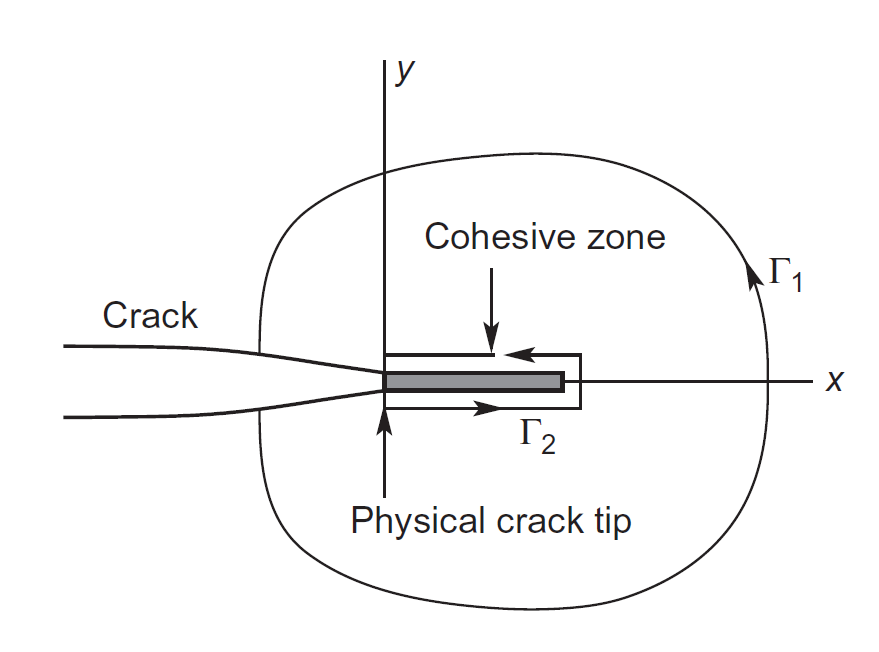
\includegraphics{../images/cohesive_zone.PNG}
\end{frame}

\begin{frame}{traction separation}
\protect\hypertarget{traction-separation}{}
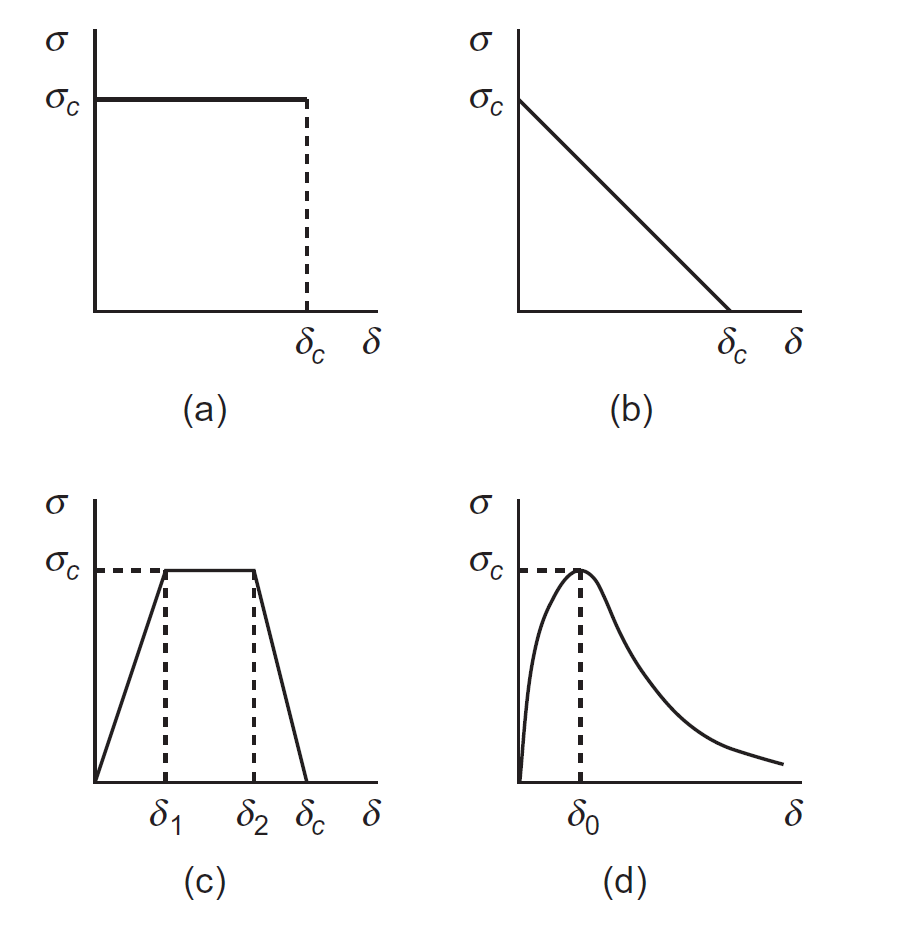
\includegraphics{../images/traction_separation.PNG}
\end{frame}

\begin{frame}{cohesive zone uses}
\protect\hypertarget{cohesive-zone-uses}{}
\begin{itemize}
\tightlist
\item
  In practice, the cohesive zone can be used to model crack growth
\item
  It is most often used to model de-bonding of adhesives
\item
  Also commonly used to model delamination in composites
\end{itemize}
\end{frame}

\begin{frame}{dcb}
\protect\hypertarget{dcb}{}
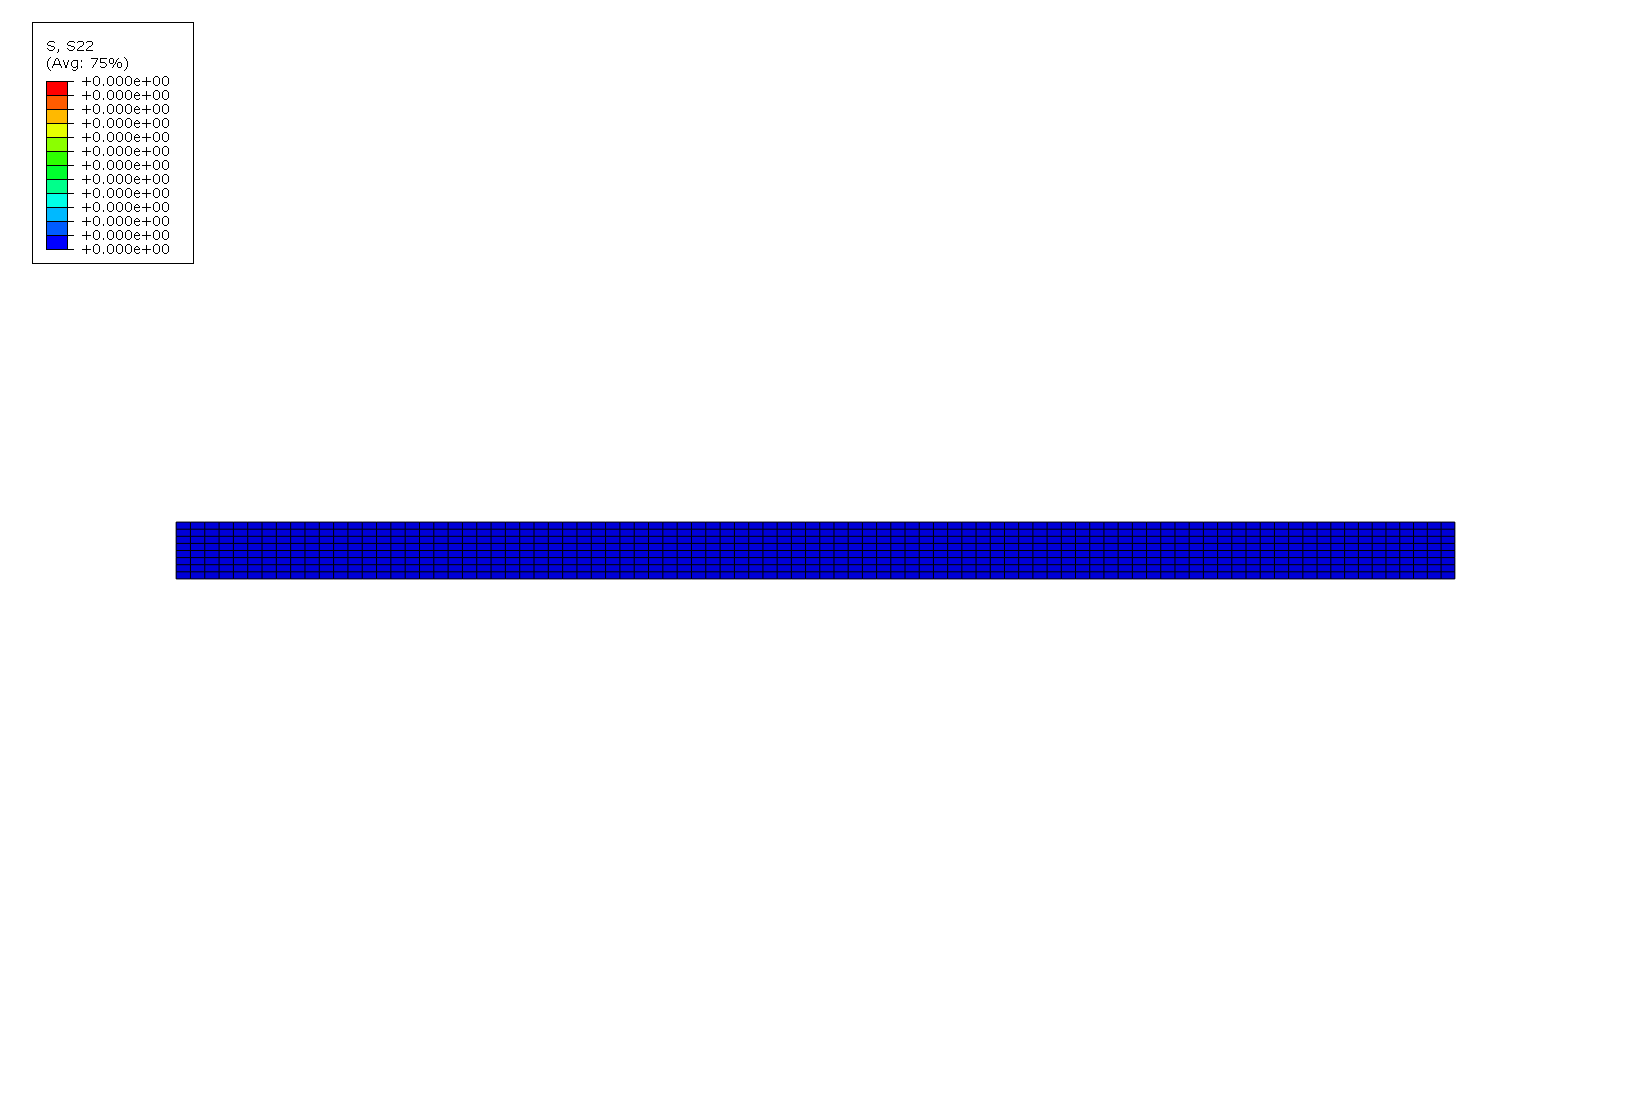
\includegraphics{../images/dcb1.png}

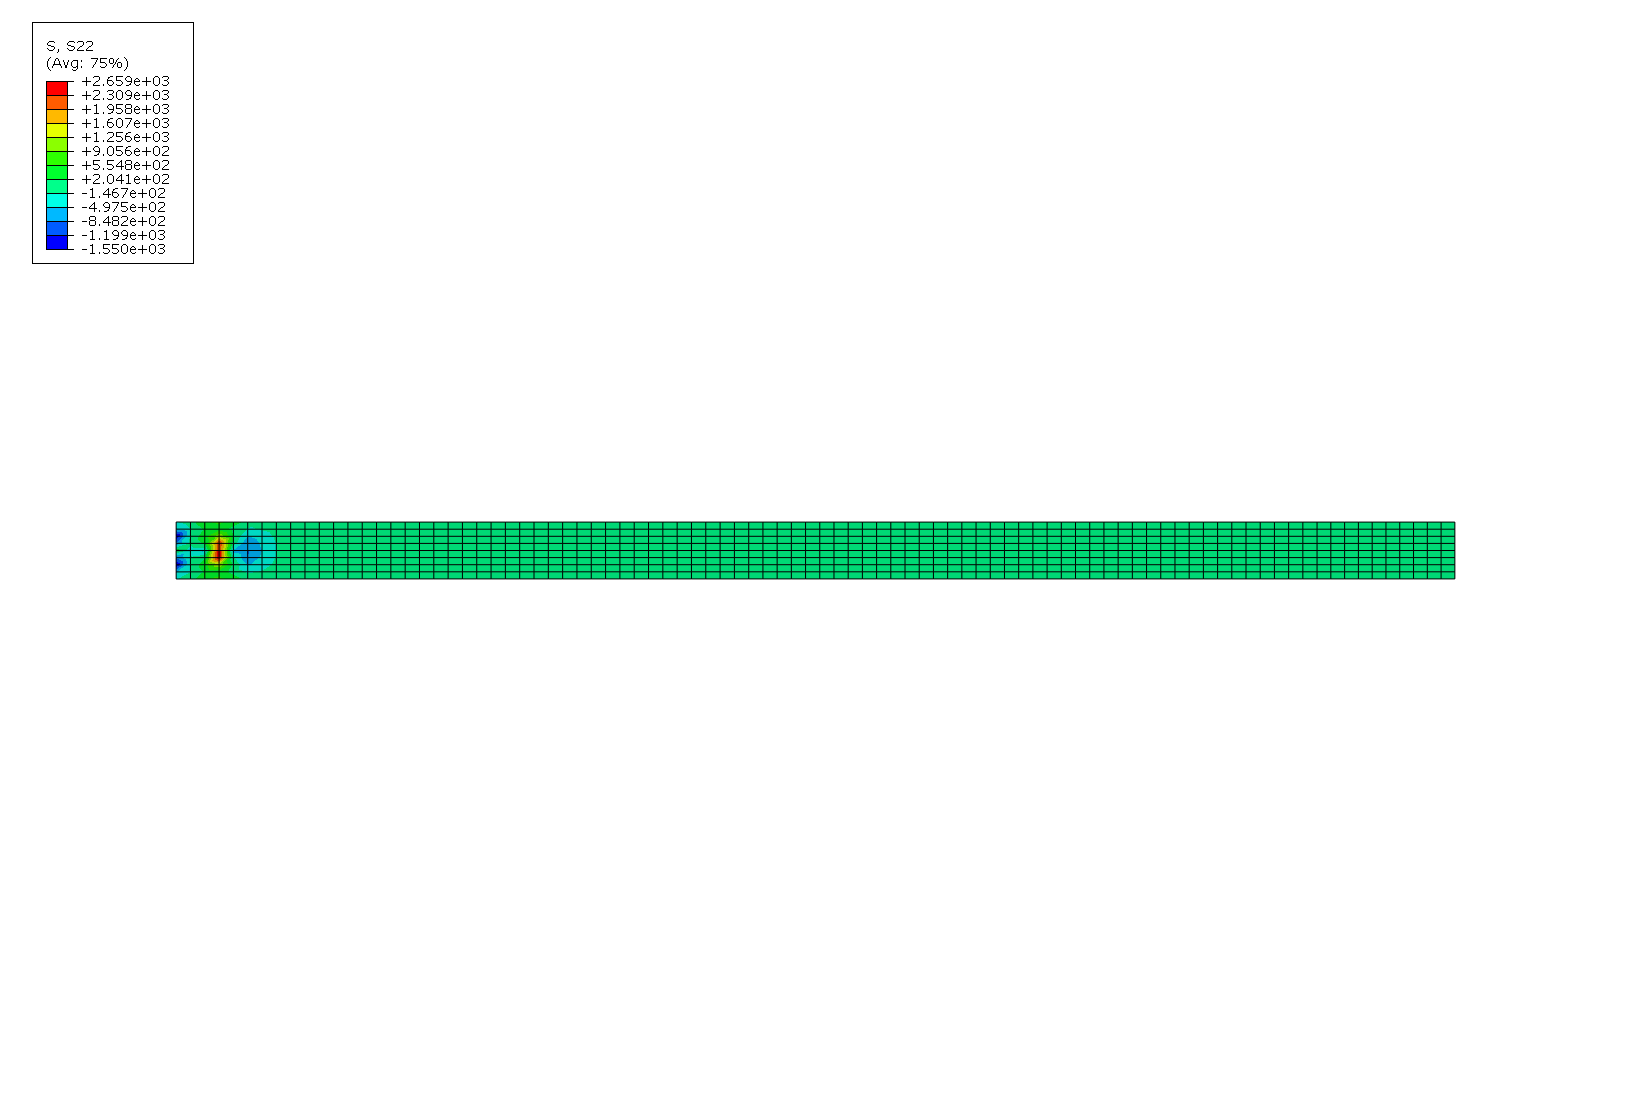
\includegraphics{../images/dcb2.png}

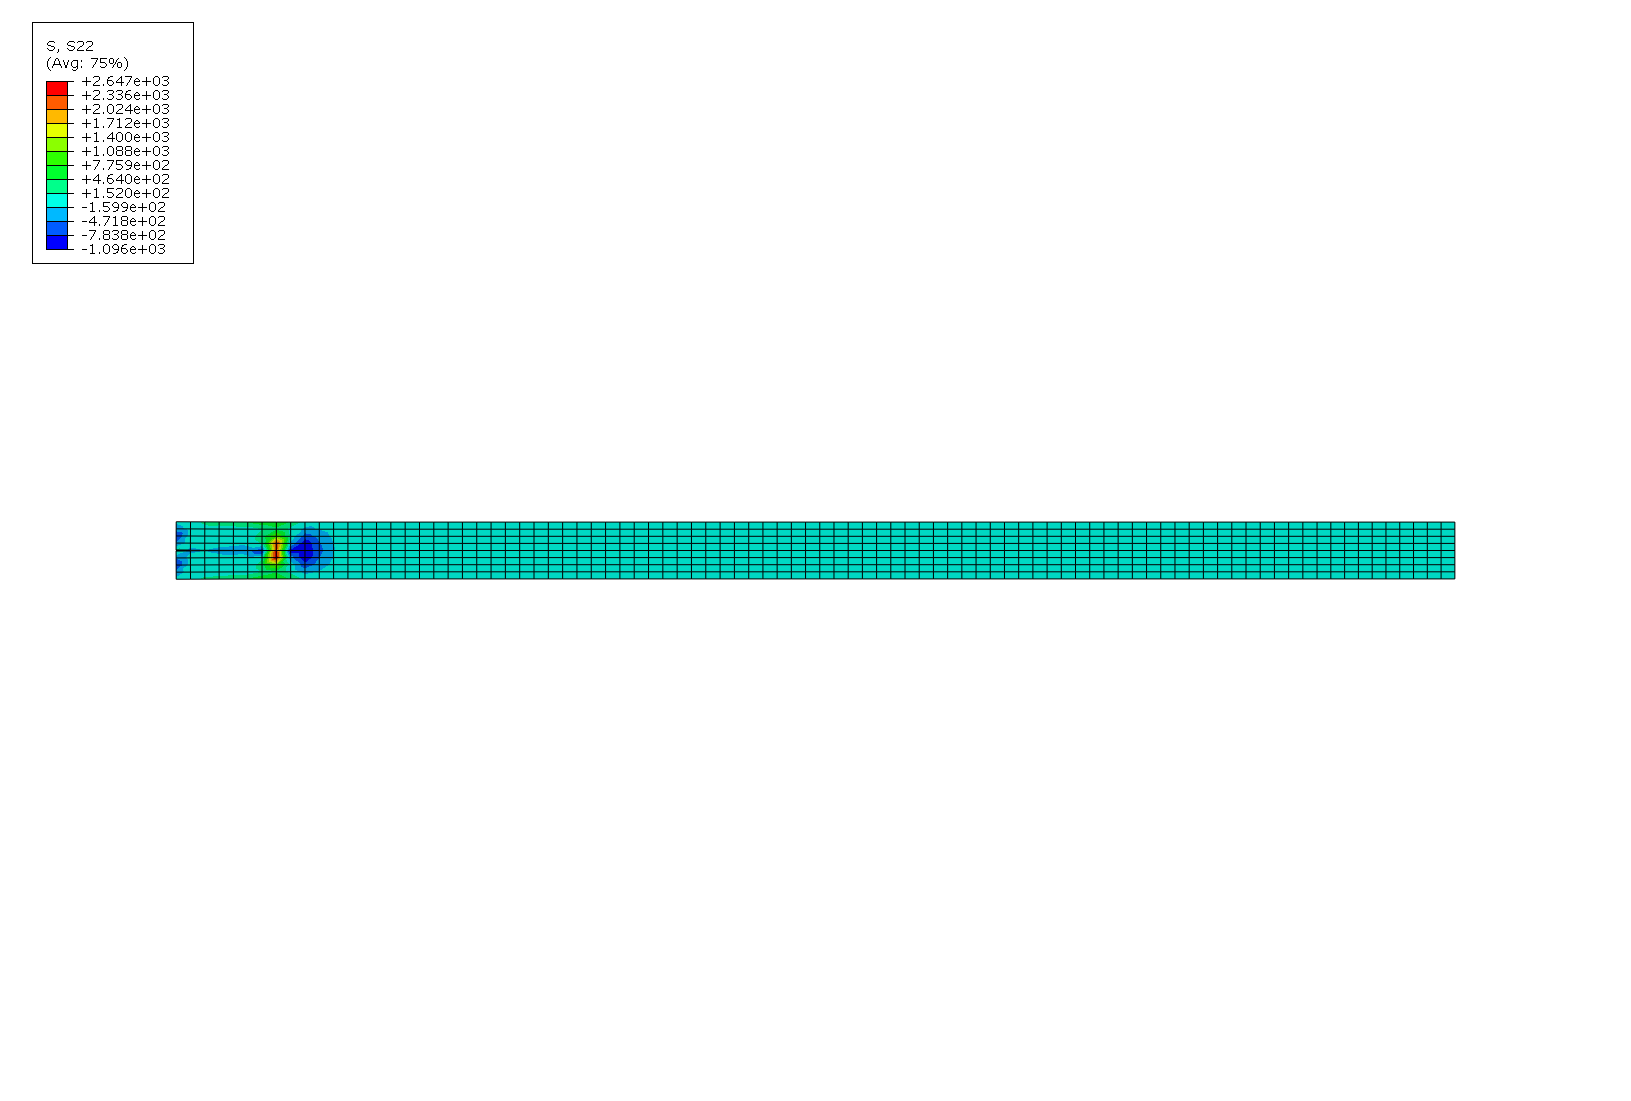
\includegraphics{../images/dcb3.png}

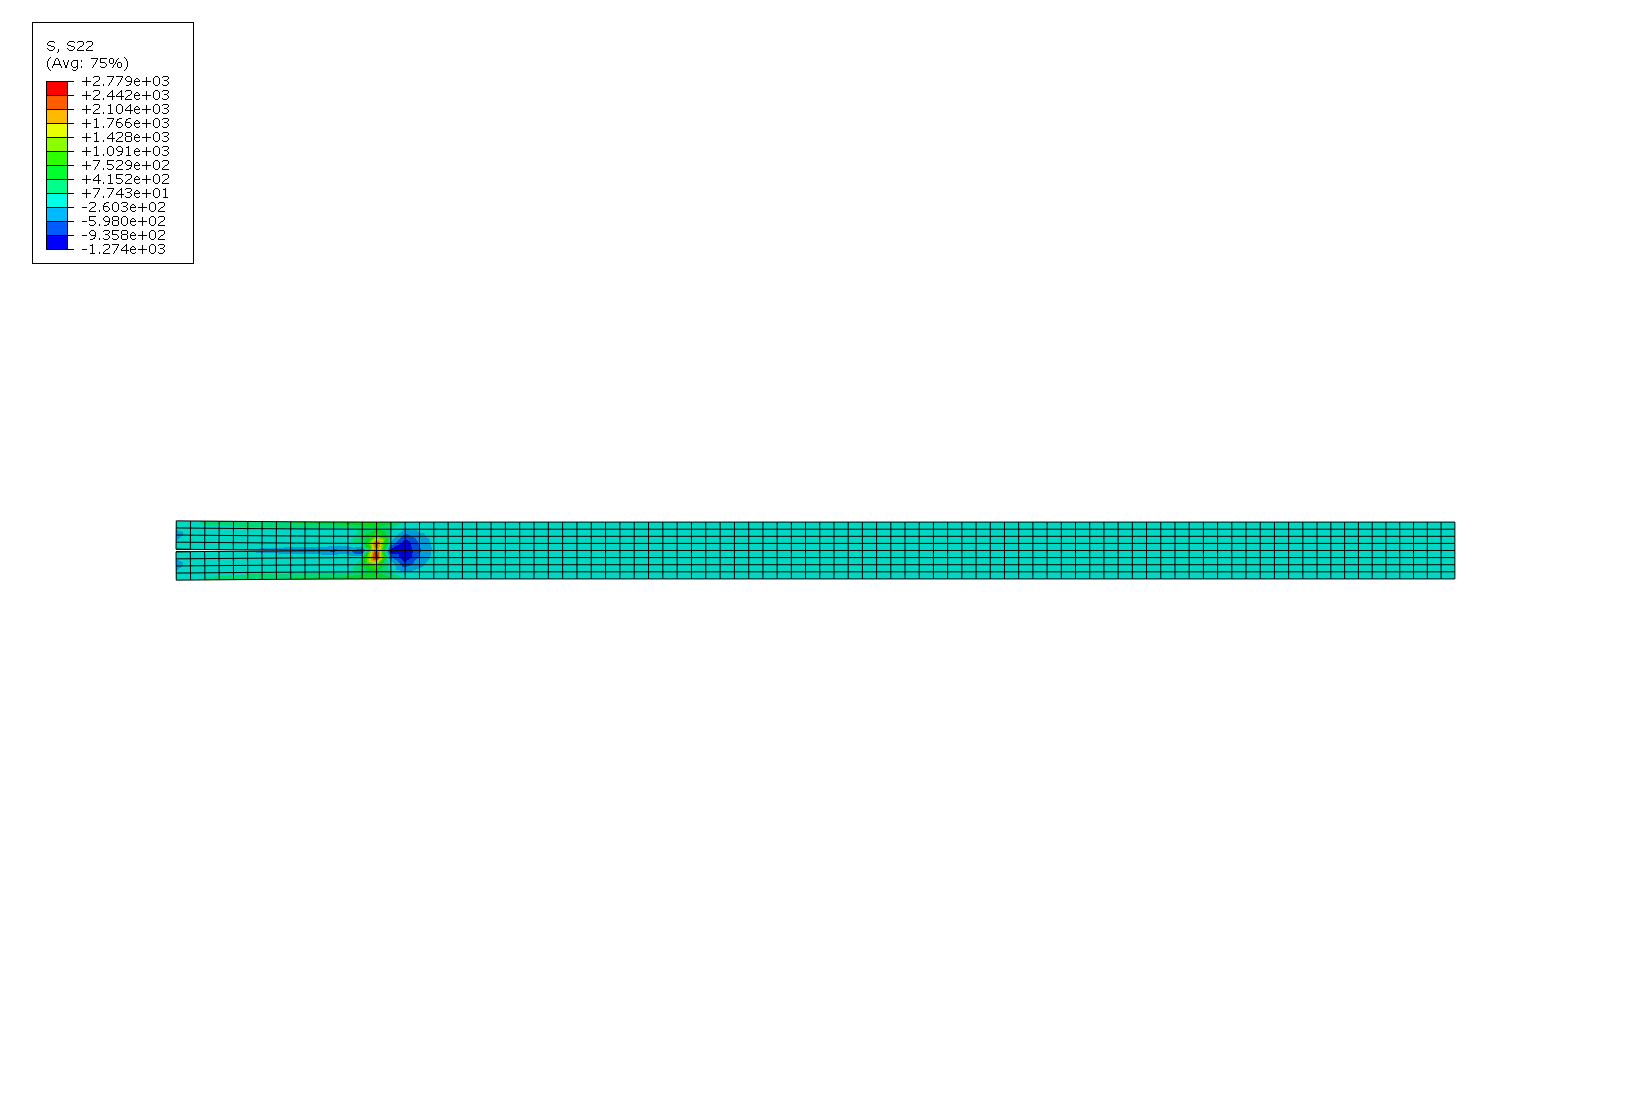
\includegraphics{../images/dcb4.png}

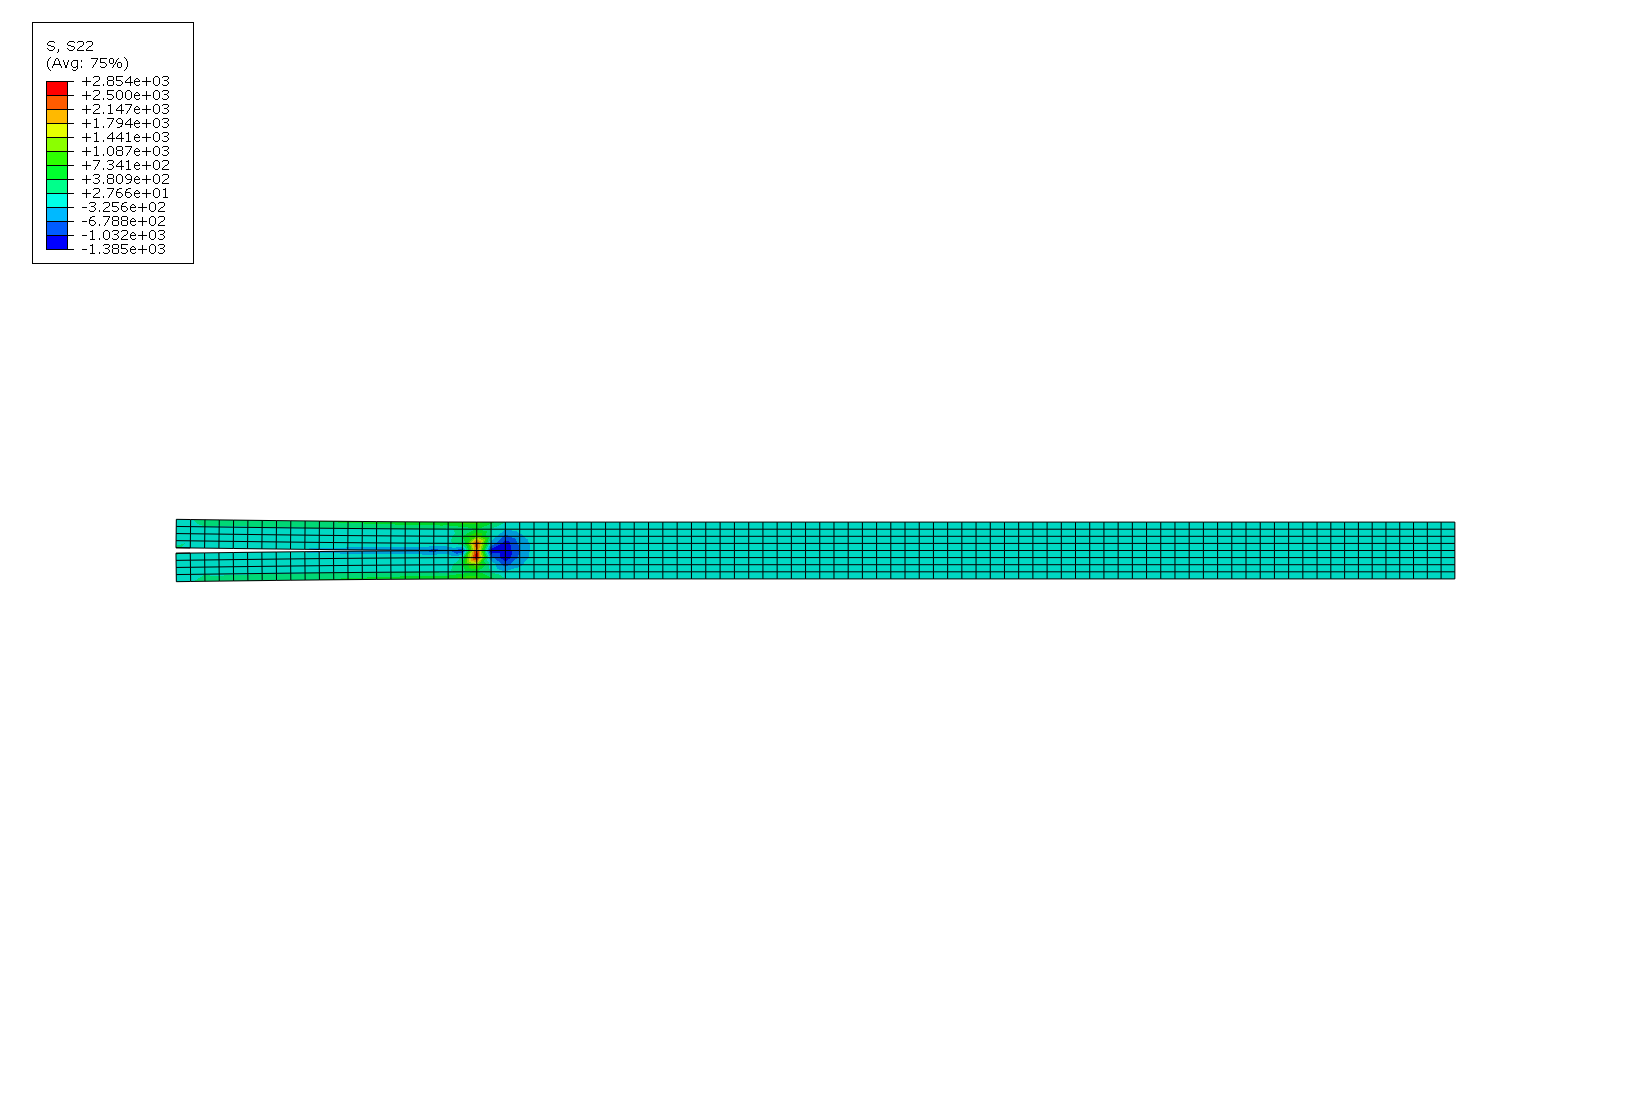
\includegraphics{../images/dcb5.png}

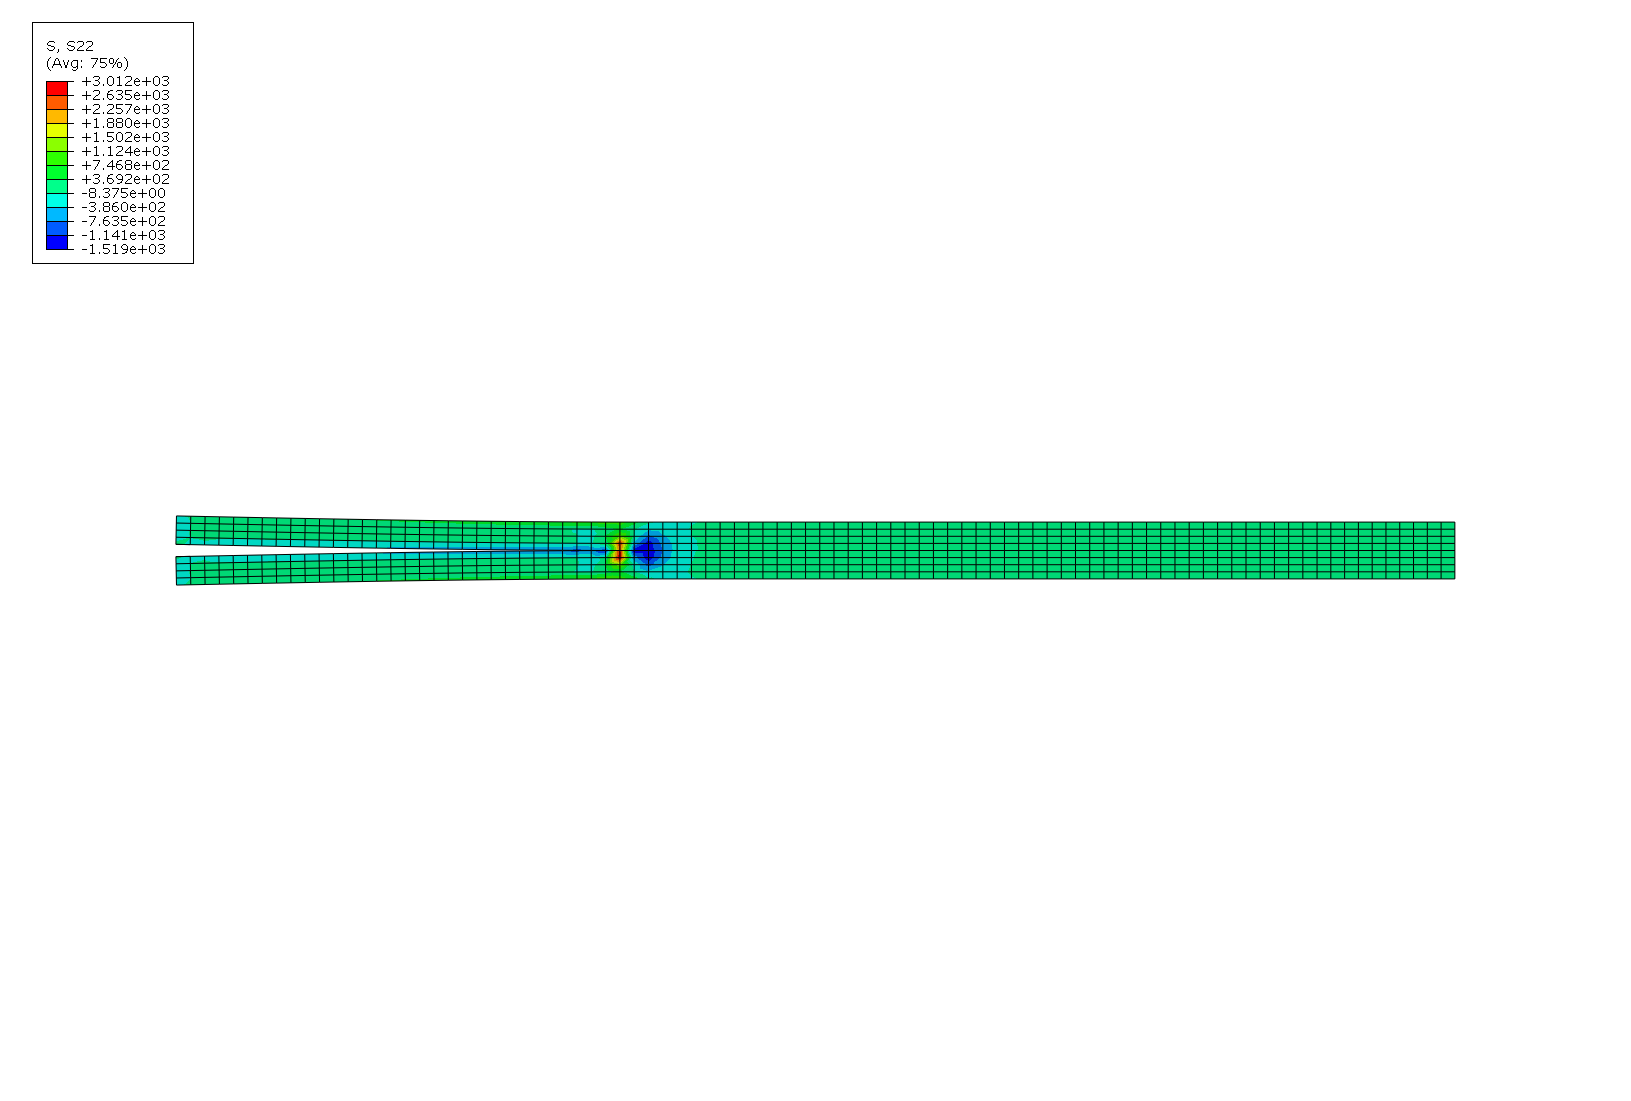
\includegraphics{../images/dcb6.png}

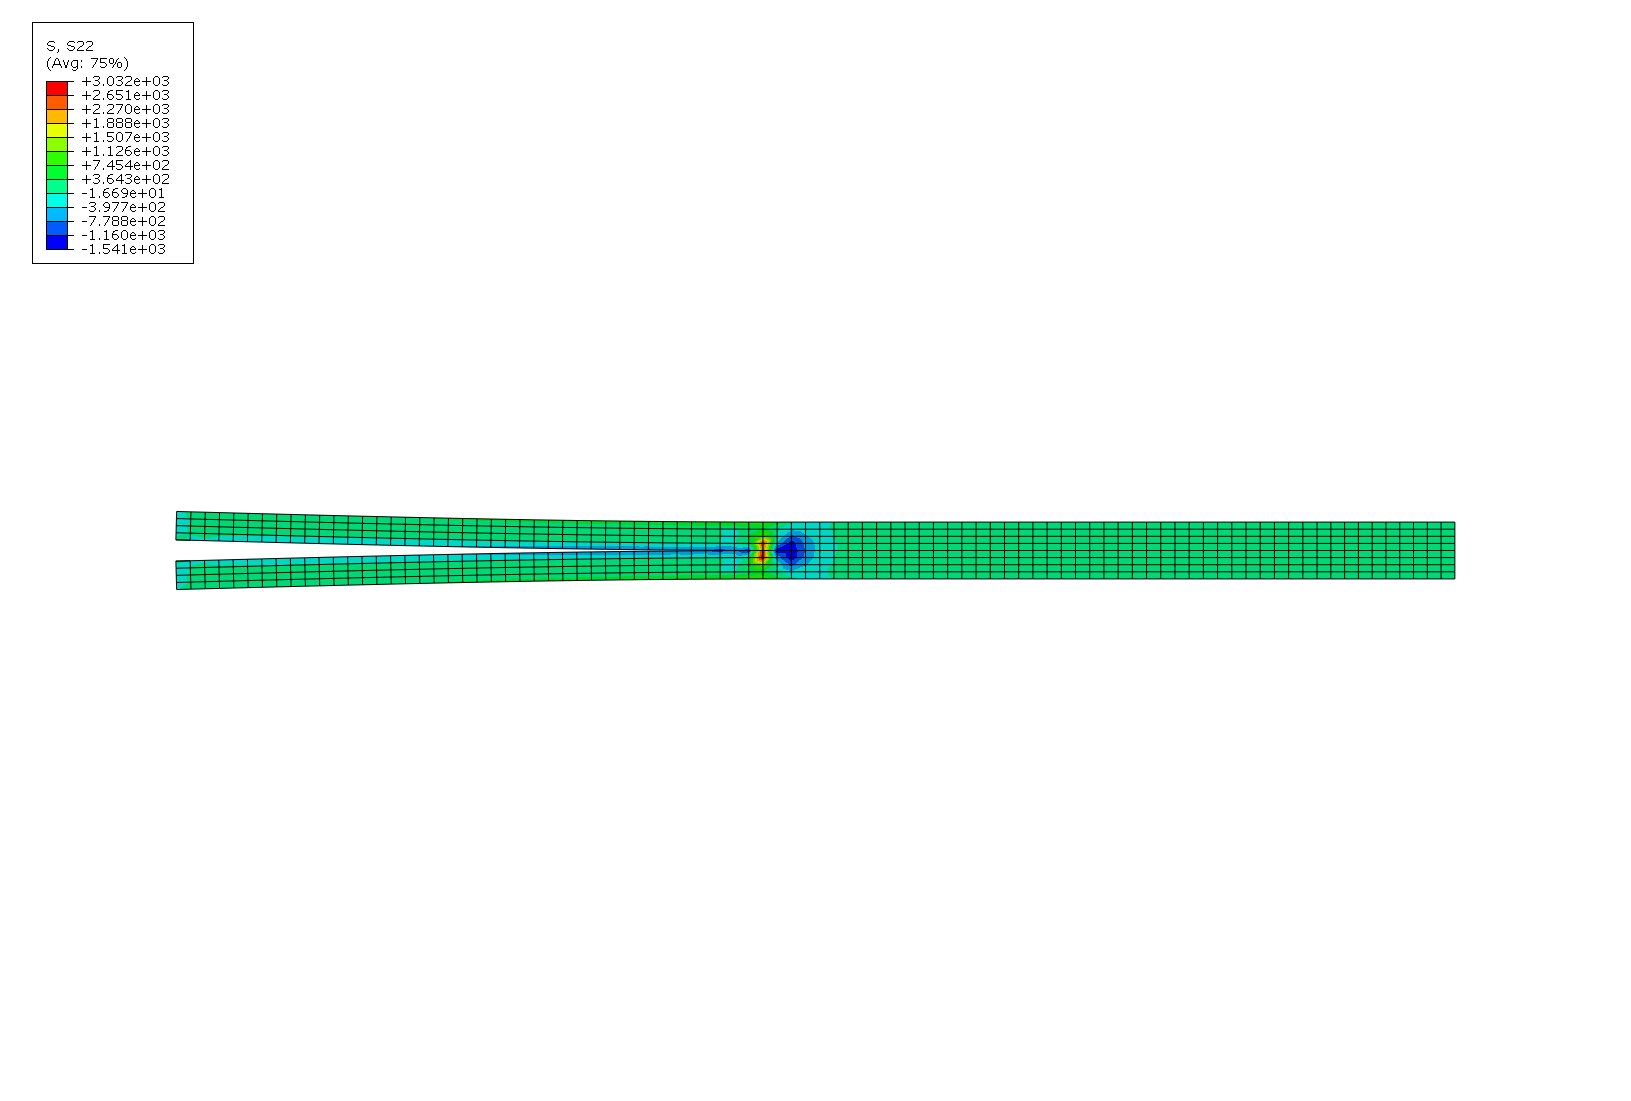
\includegraphics{../images/dcb7.png}

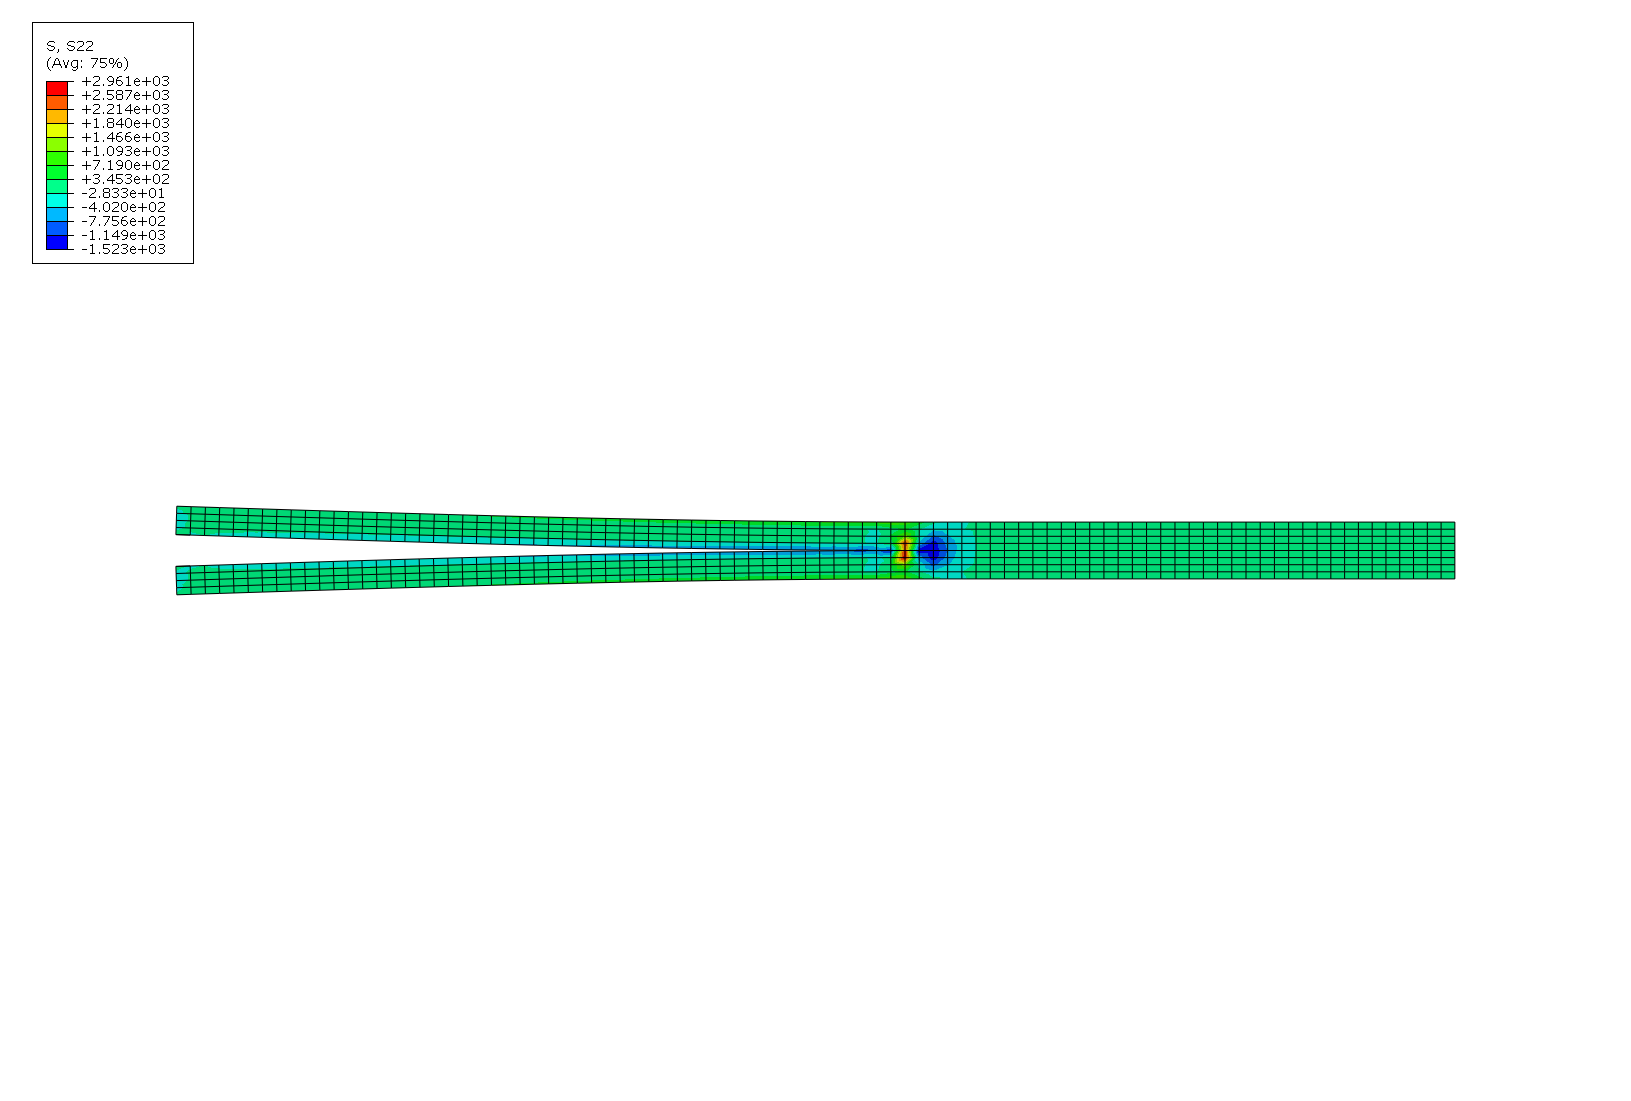
\includegraphics{../images/dcb8.png}

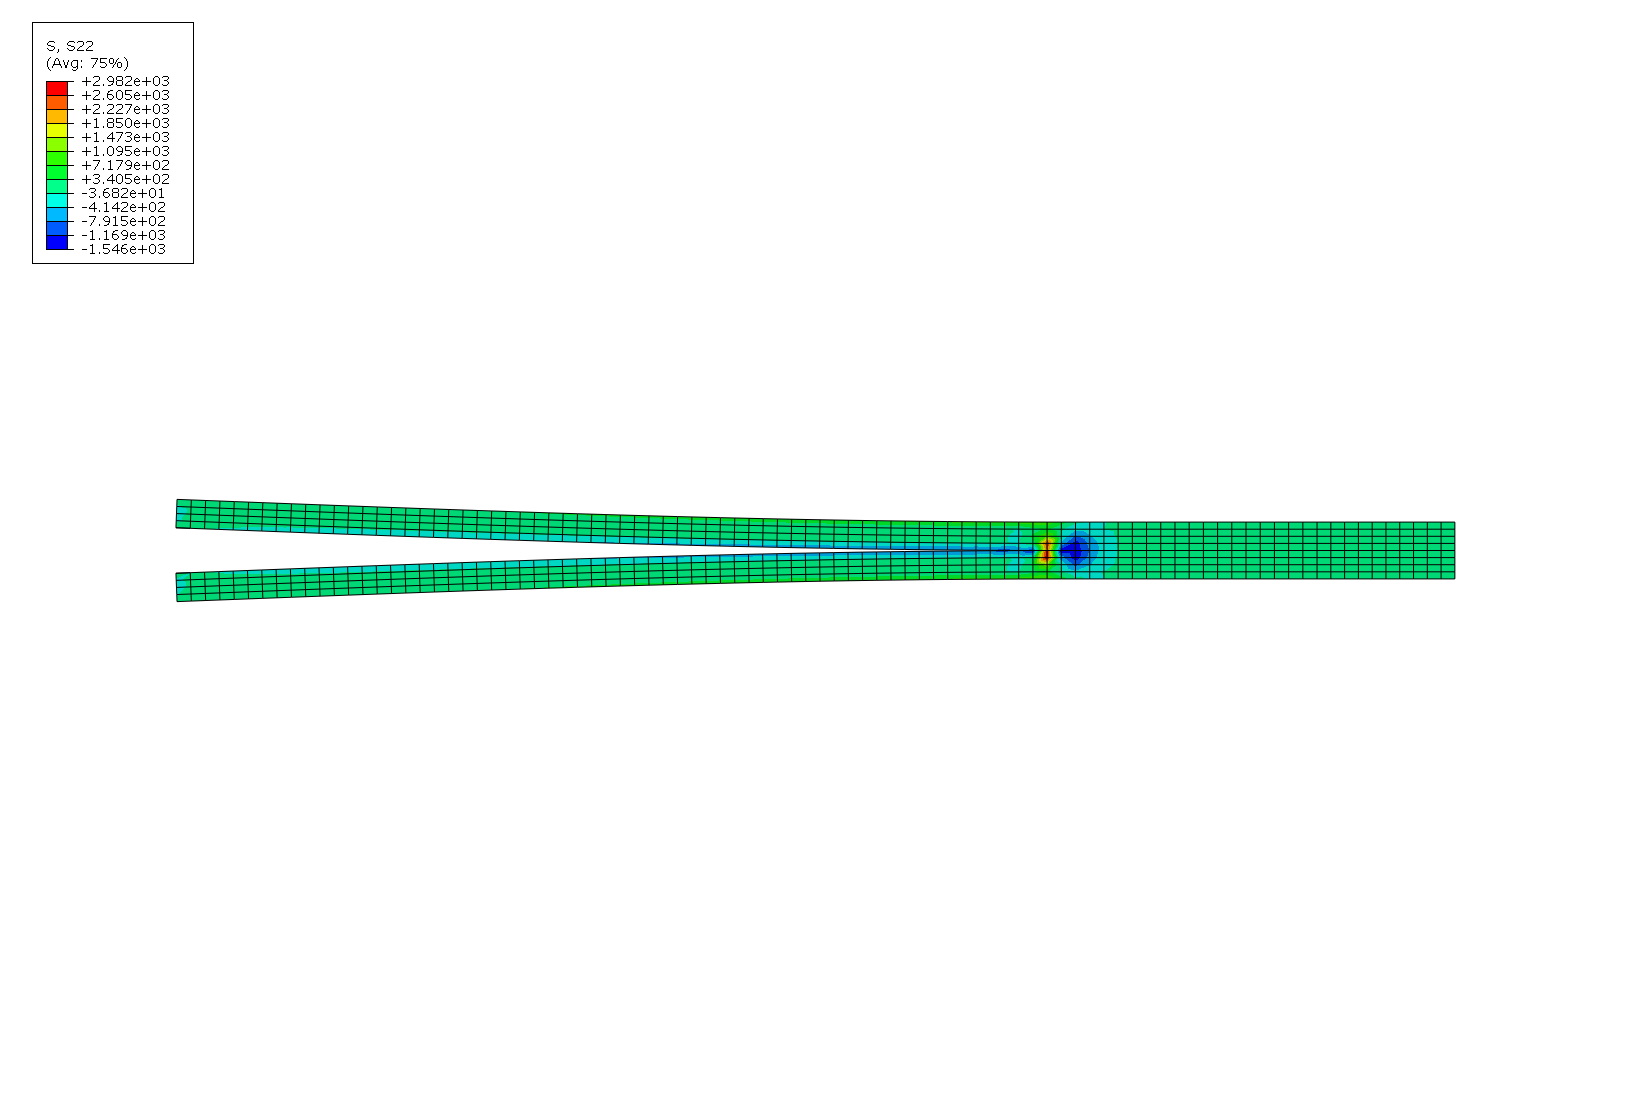
\includegraphics{../images/dcb9.png}

:::
\end{frame}

\begin{frame}{single crack}
\protect\hypertarget{single-crack}{}
\begin{itemize}
\tightlist
\item
  To solve the problem of many cohesive cracks in an RVE, we first
  consider the case of a single crack
\item
  For a crack under a uniform tri-axial stress, we consider the
  superposition 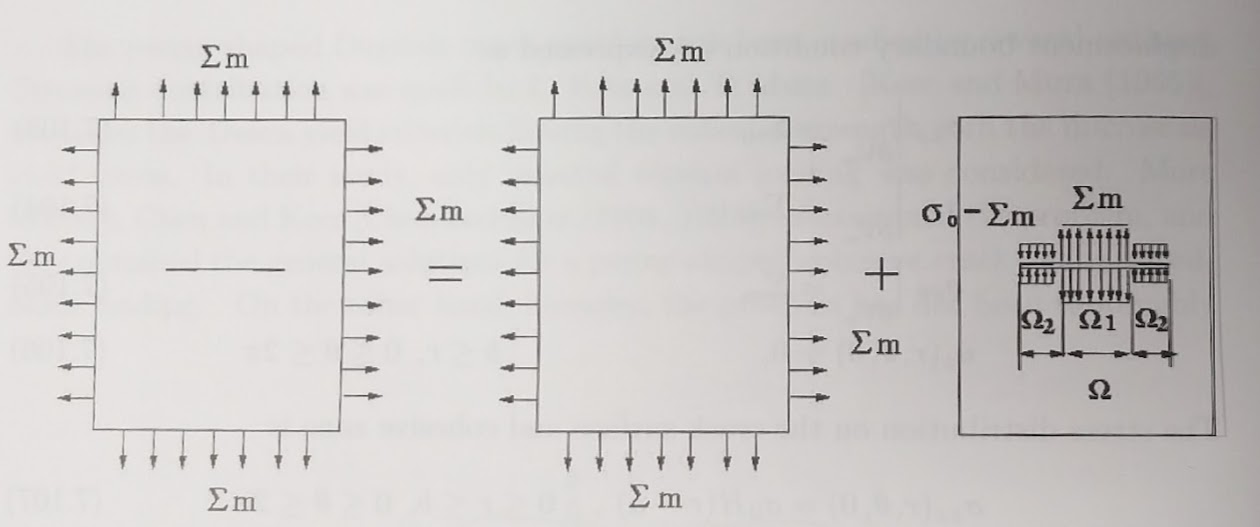
\includegraphics{../images/superposition.jpg}
\end{itemize}
\end{frame}

\begin{frame}{cohesive stress}
\protect\hypertarget{cohesive-stress}{}
\begin{itemize}
\tightlist
\item
  The cohesive stress, \(\sigma_0\) can be found as
\end{itemize}

\[\frac{\sigma_0}{\Sigma_m} = \frac{1+\sqrt{\left(\frac{4}{1-2\nu^*}\frac{\sigma_YS}{\Sigma_m}\right)^2-3}}{4}\]
\end{frame}

\begin{frame}{macro strain}
\protect\hypertarget{macro-strain}{}
\begin{itemize}
\tightlist
\item
  The macro strain tensor is not necessarily the volume average
\item
  This is due to the discontinuities (cracks)
\item
  The macro stress is the volume average (crack surfaces are traction
  free)
\end{itemize}
\end{frame}

\begin{frame}{macro strain}
\protect\hypertarget{macro-strain-1}{}
\begin{itemize}
\tightlist
\item
  One technique for finding the macro strain involves finding some
  additional strain term
\end{itemize}

\[ \varepsilon_{ij} \epsilon_{ij}^0 + \epsilon_{ij}^(add)\]

\begin{itemize}
\tightlist
\item
  Where \(\epsilon_{ij}^0 = D_{ijkl} \sigma_{kl}\) and
  \(\epsilon_{ij}^{(add)} = H_{ijkl} \sigma_{kl}\)
\end{itemize}
\end{frame}

\begin{frame}{additional strain}
\protect\hypertarget{additional-strain}{}
\begin{itemize}
\tightlist
\item
  The additional strain is given by
\end{itemize}

\[\epsilon_{ij}^{(add)} = \frac{4f(1-\nu^*)\Sigma_m\delta_{ij}}{3\beta \pi \mu^* \sqrt{1-\left(\frac{\Sigma_m}{\sigma_0}\right)^2}}\]

\begin{itemize}
\tightlist
\item
  Where \(\beta\) is the ratio between the volume of the physical crack
  and the volume of the cohesive crack and \emph{f} is the effective
  volume fraction of cracks
\item
  While cracks are assumed to be ``penny-shaped'' disks, their volume is
  treated as spherical for these purposes
\end{itemize}
\end{frame}

\begin{frame}{interaction effect}
\protect\hypertarget{interaction-effect}{}
\begin{itemize}
\tightlist
\item
  In the above calculations, properties with a * superscript an be
  calculated as either matrix or average properties
\item
  We can capture the interaction effect by using average properties
\item
  This is similar to the self-consistent model, and would need to be
  found iteratively
\item
  Note: this does not model damage growth, which is still a field of
  active research, particularly in micromechanics
\end{itemize}
\end{frame}

\end{document}
